\documentclass[border=5pt, tikz]{standalone}
\usetikzlibrary{perspective}
\usetikzlibrary{calc}
\usetikzlibrary{shadings}
\usepackage{amsmath}
\usetikzlibrary {arrows.meta,bending,positioning}
\begin{document}
 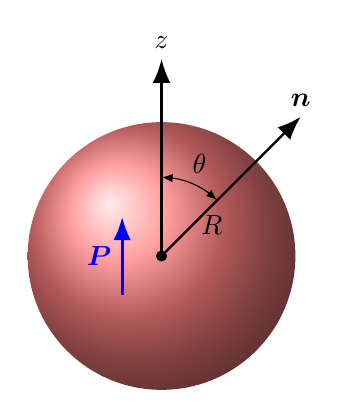
\begin{tikzpicture}

    \begin{scope}
        \coordinate (O) at (0, 0);
       

        \shade[ball color=red!50] (O) circle (17mm);

        \fill[] (O) circle (0.7mm);

        \draw [-{Latex[length=3mm]}, thick] (O) -- (0, 2.5) node [above] {$z$};
        \draw [-{Latex[length=3mm]}, thick] (O) -- ++ (45:2.5) node [above] {$\boldsymbol{n}$};
        
        \draw [latex-latex](0, 1) arc (90:45:1) node [midway, above, xshift=1mm] {$\theta$};

        \node[below] at (45:9mm) {$R$};

        % \draw [latex-latex](35:10mm) arc (35:145:10mm) node [midway, above] {$105^\circ$};

        \draw [-{Latex[length=3mm]}, very thick, blue] (-0.5, -0.5) -- (-0.5, 0.5) node [midway, left] {$\boldsymbol{P}$}; 
    \end{scope}


\end{tikzpicture}
\end{document}